\documentclass[reprint, prl, aps, showpacs]{revtex4-1}
%\documentclass[preprint, aps, showpacs]{revtex4-1}

\usepackage{graphicx}
\usepackage{amsmath,amssymb}
%\usepackage[usenames,dvipsnames]{color}
%\usepackage[colorlinks=true, citecolor=blue, linkcolor=WildStrawberry]{hyperref}
%\usepackage[citecolor=blue]{hyperref}
%\usepackage[justification=centerfirst]{caption}
\usepackage{epstopdf}

%\usepackage[latin1]{inputenc}
\usepackage{tikz}
\usetikzlibrary{shapes,arrows}

\newcommand{\braket}[2]{\left\langle#1\, |\,#2\,\right\rangle}  %  < #1 | #2 >
\newcommand{\expec}[1]{\langle#1\rangle}  %  < #1 >
\newcommand{\drm}{{\rm d}}
\newcommand{\irm}{{\rm i}}
\newcommand{\beq}{\begin{equation}}
\newcommand{\eeq}{\end{equation}}
\newcommand{\bdm}{\begin{displaymath}}
\newcommand{\edm}{\end{displaymath}}
\newcommand{\T}[1]{\tilde{#1}}
\newcommand{\wT}[1]{\widetilde{#1}}
\newcommand{\Cdot}{\!\cdot\!}
\newcommand{\SNR}{\textnormal{SNR}}
\newcommand{\rednote}[1]{{\color{red} (#1)}}
\newcommand{\fixme}[1]{\textcolor{green}{\textbf{\textit{{#1}}}}}
\newcommand{\seismon}{\textnormal{seismon}}

\DeclareFontFamily{OT1}{pzc}{}
\DeclareFontShape{OT1}{pzc}{m}{it}{<-> s * [1.10] pzcmi7t}{}
\DeclareMathAlphabet{\mathpzc}{OT1}{pzc}{m}{it}

\def\dblone{\hbox{$1\hskip -1.2pt\vrule depth 0pt height 1.6ex width 0.7pt \vrule depth 0pt height 0.3pt width 0.12em$}}

\graphicspath{{./plots/}}
\begin{document}

\title{Limiting the effects of earthquakes on gravitational-wave interferometers}

\author{Sebastien Biscans}
\affiliation{LIGO Laboratory, Massachusetts Institute of Technology, Cambridge, MA 02138, USA}

\author{Christopher Buchanan}
\affiliation{Department of Physics and Astronomy, Louisiana State University, Baton Rouge, LA 70803-4001, USA}

\author{Eric Coughlin}
\affiliation{Department of Computer Science, Luther College, 700 College Dr, Decorah, IA 52101, USA}

\author{Michael Coughlin}
\affiliation{Department of Physics, Harvard University, Cambridge, MA 02138, USA}

\author{Fred Donovan}
\affiliation{LIGO Laboratory, Massachusetts Institute of Technology, Cambridge, MA 02138, USA}

\author{Paul Earle}
\affiliation{United States Geological Survey, Golden, CO 80401, USA}

\author{Jeremy Fee}
\affiliation{United States Geological Survey, Golden, CO 80401, USA}

\author{Michelle Guy}
\affiliation{United States Geological Survey, Golden, CO 80401, USA}

\author{Matthew Perry}
\affiliation{United States Geological Survey, Golden, CO 80401, USA}

\author{Jan Harms}
\affiliation{INFN, Sezione di Firenze, Sesto Fiorentino, 50019, Italy}

\author{Nikhil Mukund}
\affiliation{Inter-University Centre for Astronomy and Astrophysics , Ganeshkhind, Pune University Campus
Pune 411 007, India}

\begin{abstract}

Astronomical detectors, which include conventional large-scale telescopes as well as second-generation ground-based gravitational wave interferometers, are susceptible to teleseismic events. In this work, we describe an early warning system for current gravitational-wave observatories based on current earthquake notification technology. We demonstrate its efficacy and test its performance on current gravitational-wave detectors.

\end{abstract}

\maketitle

\section{Introduction}
\label{sec:Intro}

Earthquakes are a significant issue for gravitational-wave detectors. In previous work \cite{CoSt2015}, we described how large-scale astronomical experiments, such as meter class telescopes and gravitational-wave interferometers, are susceptible to earthquakes. In the case of telescopes, the predominant concern was the potential for nearby, devastating earthquakes which will damage either the surrounding structure or the mirrors that make up the telescope. We argued that a regional early earthquake warning (EEW) \cite{Al2012,KuAl2013a,KuAl2013b,KuHe2014,CoLa2009a,CoLa2009b,BoAl2014,HoKa2008} system was important to minimize potential damage to telescopes. 
Gravitational-wave detectors, on the other hand, are susceptible to teleseismic events from around the world \cite{MaFa2012}. 
The Laser Interferometer Gravitational-wave Observatory (LIGO) \cite{aligo}, Virgo \cite{avirgo}, and GEO600 \cite{Gr2010} detectors are part of a network of gravitational-wave interferometers that have made the first direct observations of gravitational waves \cite{AbEA2016a,AbEA2016e}. These detectors can be destabilized by significant ground motion, despite seismic isolation systems designed to minimize such effects \cite{AbAd2002,StAb2009}.

During the last LIGO science run, large amplitude earthquakes from around the world would typically cause the detectors to fall out of lock \cite{CoSt2015}. Not only were the data around the time of the earthquake not useful for gravitational-wave detection, but it would also take hours of dead time for the detectors to return to the locked state. 
We showed that there are potential gains to be made with an early warning system assuming that the incurred downtime could be reduced with sufficient advance notice of the earthquakes' arrivals.
Detailed studies of earthquake response during S5 and S6 showed that there is about one teleseismic event each week producing ground motion at the sites too strong for the control system to be able to maintain lock. In most cases, it was then impossible to lock the interferometer for some hours. A scheme that would suppress disturbances of earthquakes early in the isolation system with the final goal to maintain lock during strong ground motion, even at the price of increased instrumental noise, could potentially lead to substantial increase of the duty cycle. This will likely be of greater importance even in high-power configurations of the advanced detectors, where thermalization of test masses during the locking procedure could potentially increase the time it takes to reach maximal sensitivity.

For this reason, we have created an earthquake early warning client using a real-time event messaging system of the US Geological Survey. The messages contain information about the fault rupture such as location, depth, magnitude. They are received and processed in real time to estimate arrival times, and seismic amplitudes of the various seismic phases at the detector sites. In addition, it is important to investigate how the client can be implemented. Finally, further effort needs to be spent on investigating the effect of strong ground motion on the aLIGO control system, and to develop methods for adapting the controls as a means of ``riding out the earthquake''.

In this paper, we will describe \seismon, a code developed to mitigate the effects of teleseismic events on ground-based gravitational-wave detectors. It uses event notices received from USGS and makes time of arrival, and amplitude predictions are made for earthquake seismic wave phases at sites of current detectors. Using a combination of earthquake magnitude, distance, and depth information, a prediction of the likelihood of the earthquake causing data disruption at the sites is made.
%In section~\ref{sec:algorithm}, we describe the algorithm.
%In section~\ref{sec:performance}, we describe the performance of the algorithm on the most recent gravitational-wave detector data.
%In section~\ref{sec:conclusions}, we offer concluding remarks and suggest directions for future research.

\section{Algorithm}
\label{sec:algorithm}

Figure~\ref{fig:flowchart} shows the flowchart for the \seismon pipeline, developed to mitigate the effects of teleseismic events on ground-based interferometric gravitational wave detectors. It uses event notices received from USGS and makes time of arrival and amplitude predictions for earthquake seismic wave phases at sites of current detectors. Using a combination of earthquake magnitude, distance, and depth information, a prediction of the likelihood of the earthquake causing data disruption at the sites is made.

% Define block styles
\tikzstyle{decision} = [diamond, draw, fill=blue!20,
    text width=4.5em, text badly centered, node distance=3cm, inner sep=0pt]
\tikzstyle{block} = [rectangle, draw, fill=blue!20,
    text width=5em, text centered, rounded corners, minimum height=3em]
\tikzstyle{line} = [draw, -latex']
\tikzstyle{cloud} = [draw, ellipse,fill=red!20, node distance=3cm,
    minimum height=2em]
\tikzstyle{emptyblock} = [rectangle, minimum height=3em]

\begin{figure}[t]
 \begin{center}
 \begin{tikzpicture}[node distance = 2.3cm, auto]
    % Place nodes
    \node [emptyblock] (init) {};
    \node [block, left of=init] (PDL) {PDL};
    \node [block, right of=init] (GeoJSON) {GeoJSON};
    \node [block, below of=init] (Parse) {Parse events};
    \node [block, below of=Parse] (Traveltimes) {Calculate travel times};
    \node [block, below of=Traveltimes] (XML) {Produce XML files};
    \node [block, below of=PDL, node distance=9cm] (Plot) {Summary / Plot};
    \node [block, below of=GeoJSON, node distance=9cm] (Rsync) {Rsync};
    \node [block, below of=Rsync] (Epics) {Epics Channel};
    % Draw edges
    \path [line] (PDL) -- (Parse);
    \path [line] (GeoJSON) -- (Parse);
    \path [line] (Parse) -- (Traveltimes);
    \path [line] (Traveltimes) -- (XML);
    \path [line] (XML) -- (Plot);
    \path [line] (XML) -- (Rsync);
    \path [line] (Rsync) -- (Epics);
 \end{tikzpicture}
 \end{center}
 \caption{A flow chart of the \seismon pipeline.}
 \label{fig:flowchart}
\end{figure}

\subsection{Notices}

\seismon relies on the most preliminary notices of earthquakes currently available generated by worldwide networks of seismometers. 
In general, the process of identification occurs when a primary or P-wave arrival is identified in a number of nearby seismometers.
Preliminary estimates of the location, including latitude, longitude, and depth, are then derived by triangulating these arrivals. 
Earthquake magnitude estimates, which will also couple into the ground velocity at the gravitational-wave detectors, come later.
This is due to the necessity of estimating the distance a fault moved and the force required to move it.
Potential warning times becomes a question of how fast P-waves travel relative to secondary or S-waves and surface waves, which travel between 3-6\,km/s for S-waves and slightly slower for surface waves. These are more important to gravitational-wave detectors due to their higher amplitude.

The United States Geological Survey (USGS) provides a number of channels for information about earthquakes, on different time-scales. 
The earliest, which we will use in the pipeline, are automated pipelines which use USGS-supported worldwide networks of seismometers to make earthquake identifications. 
The earliest solutions provide event source parameters, including both location and magnitude estimates.
At later times, seismometer specific phase, amplitude and magnitude parameters are provided.
Furthermore, moment tensor solutions and finite fault models are calculated from the array data.
These solutions are distributed through USGS's Product Distribution Layer (PDL), which has been configured to receive all notifications of earthquakes worldwide. 
As all USGS-supported networks submit notices through this service, the pipeline is ensured to receive all relevant notices.
In particular, the notification messages are in the form of either EQXML or QuakeML Extensible Markup Language (XML) files, although the distribution also provides image files and other related content depending on the information.
Each network that detects an earthquake provides time-tagged versions of their products, which will allow us to estimate the delay induced by the process of earthquake identification and product distribution.
This is a cross-platform Java based code that runs constantly on a dedicated machine. 

\begin{figure}[t]
\hspace*{-0.5cm}
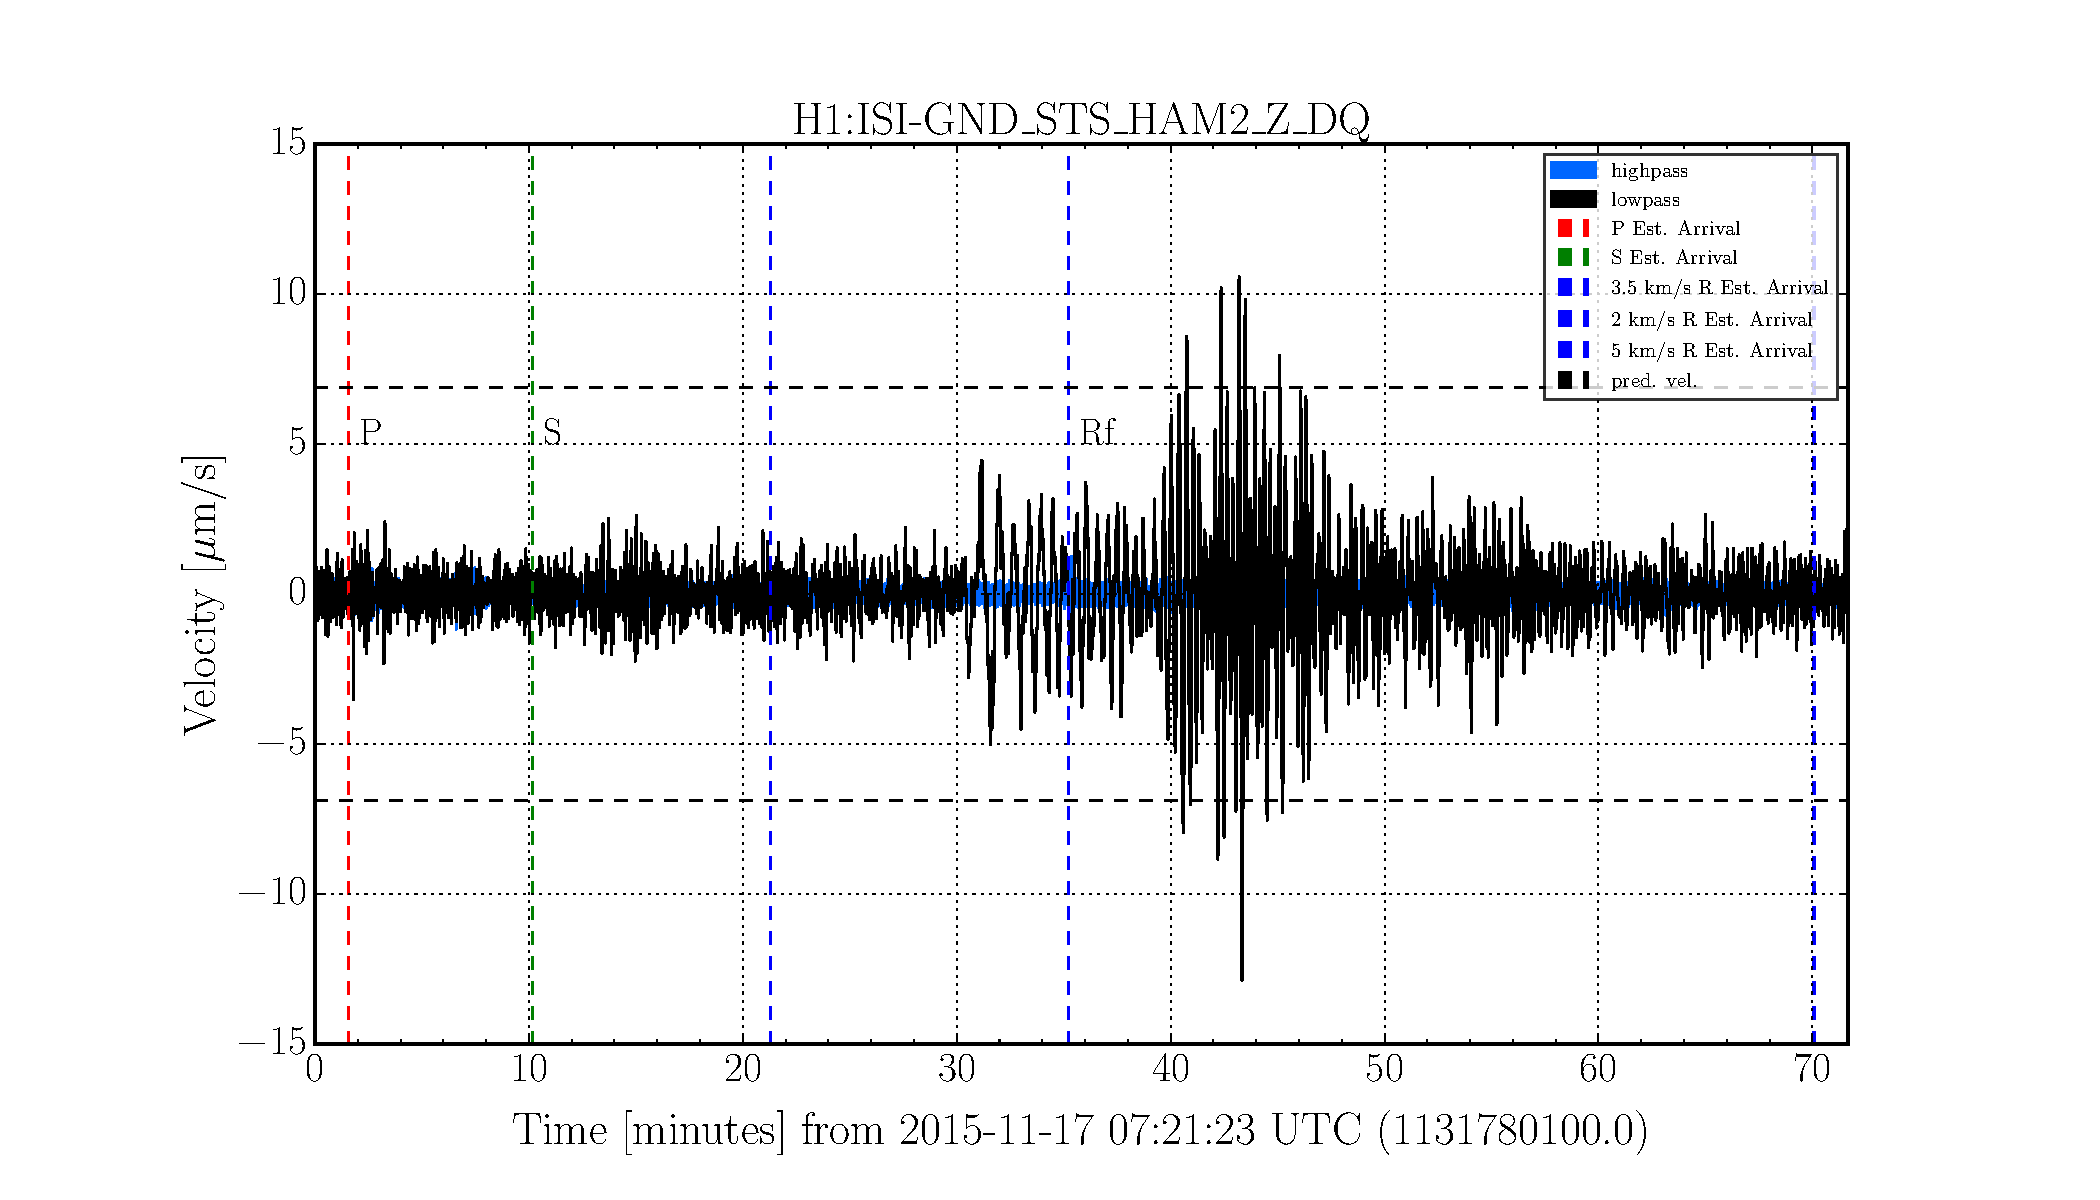
\includegraphics[width=3.5in]{timeseries.pdf}
\caption{Time-series of ground motion data from recent earthquake. The plot on the left is the ground motion from a seismometer at the LIGO Hanford site located in Washington, USA for the Nov 17, 2015 6.5 magnitude earthquake in Greece. The P, S, and surface waves all have distinctive arrivals in this case. The surface waves are shown to last tens of minutes.}
 \label{fig:timeseries}
 \end{figure}

\subsection{Analysis}

The second step of the process is to convert event notifications to information about the time of arrival and amplitudes at the sites.
In summary, we use the location and magnitude estimates the PDL client for two purposes. 
The first is the time of seismic wave arrivals at the gravitational-wave detectors.
The second is the ground motion at the gravitational-wave detectors.
Accurate prediction of the ground velocity amplitude based on earthquake magnitude and distance will be required to limit the false alarms. 
This equation should account for physical effects with variable parameters used to fit to the seismic data currently available.
P- and S-wave arrivals can be accurately determined given latitude, longitude, and depth information by calculating travel times using the iaspei-tau package wrapped by Obspy. We can approximate surface waves as having a constant 3.5\,km/s speed values. 

The second step is to make amplitude predictions for each site. 
We estimate the peak amplitude of the surface waves, $Rf_{amp}$, at the sites using equation~\ref{eq:Rfamp}, which we describe below. This was developed as a fit to historical earthquakes at the gravitational-wave detectors.
Choosing the peak amplitude was not an arbitrary choice, especially as compared to root-mean-squared (RMS) ground-motion.
A RMS value depends on technical calculation choices, which to be effective, will depend on the event in question, which is complicated.
Eventually it would be appropriate to determine what observational quantity is best suited to predict trouble for the detectors, but for now we adopt peak amplitude due to its relative simplicity.
Both the time-of-arrivals and amplitude prediction are predicted as a function of distance. This allows users of the algorithm to interpolate these metrics for their locations of interest. In general, we generate the predictions for all currently operating gravitational-wave detectors.

\begin{figure*}[t]
\hspace*{-0.5cm}
 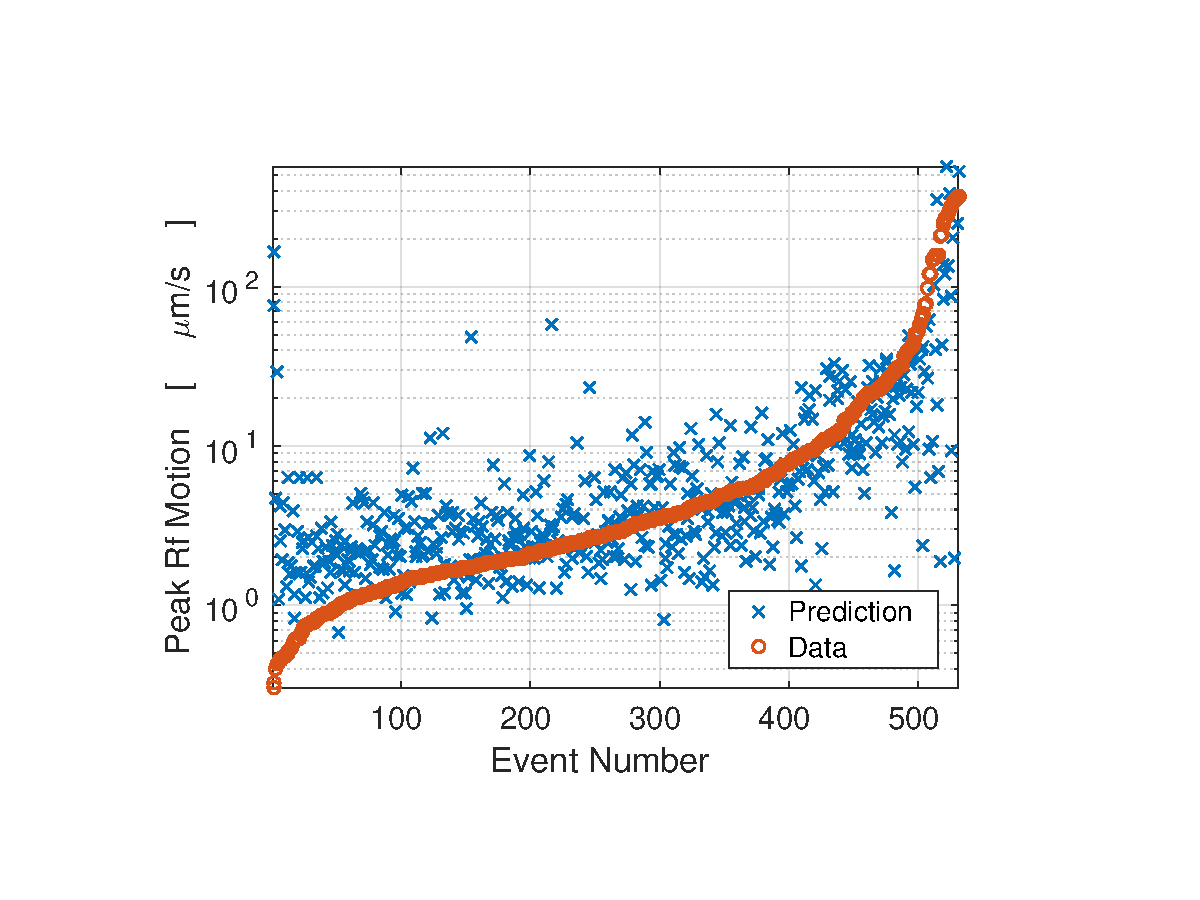
\includegraphics[width=3.5in]{Prediction_LHO_S5_S6.pdf}
 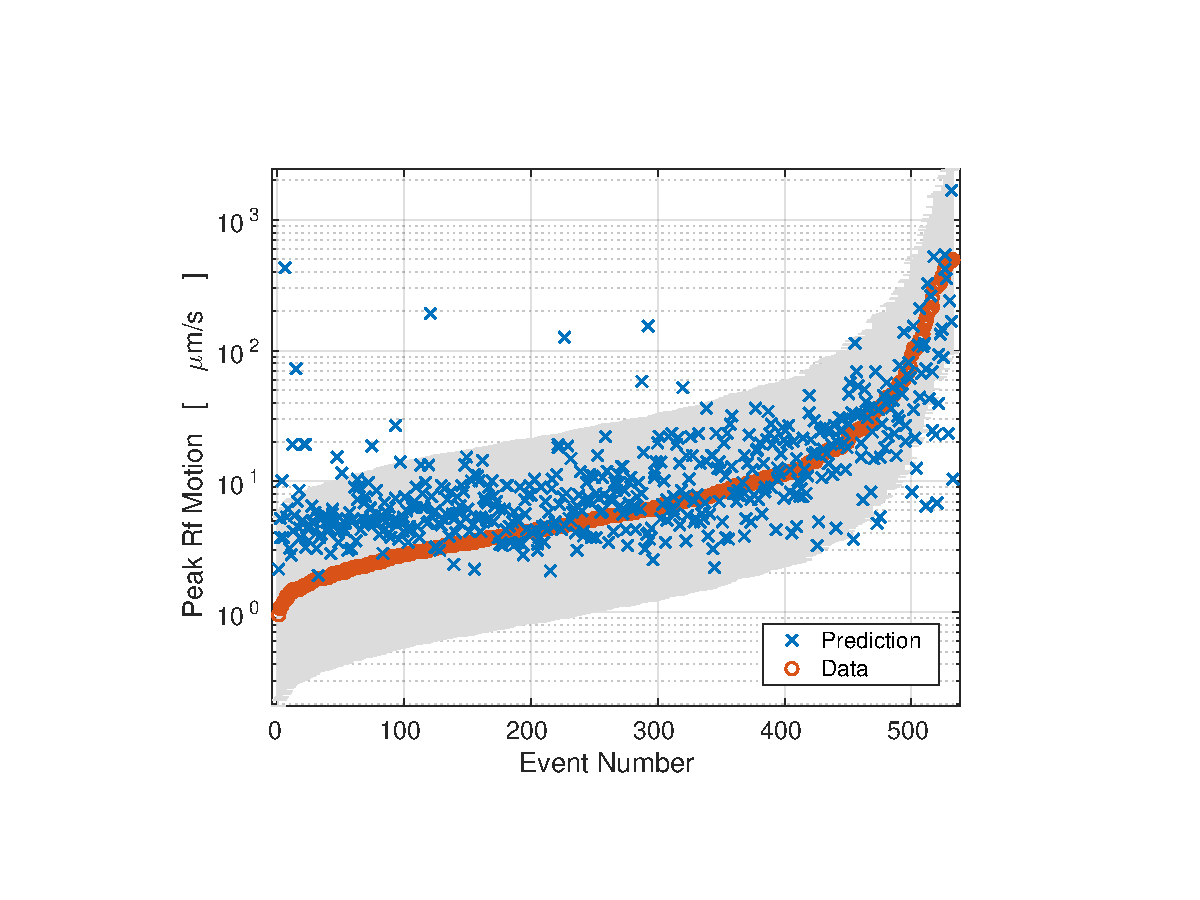
\includegraphics[width=3.5in]{Prediction_LLO_S5_S6.pdf}
 \caption{Fit of peak velocities seen during S5-S6 at the interferometers (LHO and LLO) to equation \ref{eq:Rfamp}.  Fit parameters are estimated from S5-S6 data. The events have been ordered by their measured peak ground velocity (in blue) and the green crosses correspond to the prediction from the equation. About 92\% (LHO and LLO) of events are within a factor of 5 of the predicted value.}
 \label{fig:regression}
\end{figure*}

We now examine the historical earthquake record and predict the likely ground motion seen. We then use seismic data from on site observations to predict how ground motion will affect the observatories. We have developed an equation attempting to account for physical effects with variable parameters used to fit to the data. Coupling strength of a source at a certain depth to surface Rf waves, dissipation during propagation, geometric amplitude evolution, and frequency dependent scaling of the magnitude into ground displacement were some of the terms used. A few more terms, not physically motivated, were also used to improve the fit. We estimate the amplitude of the surface waves, $Rf_{amp}$, at the sites using the equation

%Rf_{amp} = 10^{-3} *M*Af*e^{-2*pi*h*fc/cd}*e^{-2*pi*r*fc/ch/Q}/r^{rs}
\begin{equation}
Rf_{amp} = 10^{-3} M Af e^{-2 \pi h f_c/cd}/r^{rs}
\label{eq:Rfamp}
\end{equation}

where $f_c = 10^{2.3-M/2}$, $Af = \frac{Rf_0}{f_c^{Rf_s}}$, M is the magnitude of the earthquake, d is the distance, h is the depth of the earthquake, c is the speed of the surface-waves, and $f_{c}$ is the corner frequency. 
These parameters are derived from minimizing the difference between the amplitude seen at the interferometer and that predicted by the equation. 
To do so, we use a Metropolis Hastings MCMC algorithm implementing adaptive simulated annealing (SA), which statistically guarantees obtaining solutions close to global minima \cite{KiGe1983,In2000}.
These are shown for the gravitational-wave detectors in this study in Table~\ref{table:fit}. The regression is shown in Fig.~\ref{fig:regression} for both the LHO and LLO gravitational-wave interferometers. 
For LHO and LLO, the data was taken from November 2005 to October 2007 (Science Run 5) and July 2009 to October 2010 (Science Run 6).
For Virgo, the data was taken from June to September 2011 (Virgo Science Run 4).
For GEO, the data was taken from July 2010 to June 2011 (GEO High Frequency).
Figure~\ref{fig:MvsR} shows the peak ground velocity as a function of magnitude and distance for the models. Based on the above equations, we expect that earthquakes with magnitudes greater than 5 can exceed ground velocities of $1 \mu$m/s.

%$Q = \frac{Q0}{fc^{Qs}}$, 

\begin{table}[]
\centering
\label{table:fit}
\begin{tabular}{|c|c|c|c|c|}
\hline
Detector & $Rf_0$ & $Rf_s$ & $cd$ & $rs$ \\ \hline
LHO & 76.44 & 1.37 & 440.68 & 1.57 \\ \hline
LLO & 0.43 & 1.40 & 739.18 & 0.95 \\ \hline
VIRGO & 0.21 & 1.88 & 497.35 & 0.86 \\ \hline
GEO & 4.45 & 1.14 & 351.85 & 1.13 \\ \hline
\end{tabular}
\caption{Best fit parameters to the peak velocities seen at the interferometers to equation \ref{eq:Rfamp}.}
\end{table}

\begin{figure*}[t]
\hspace*{-0.5cm}
 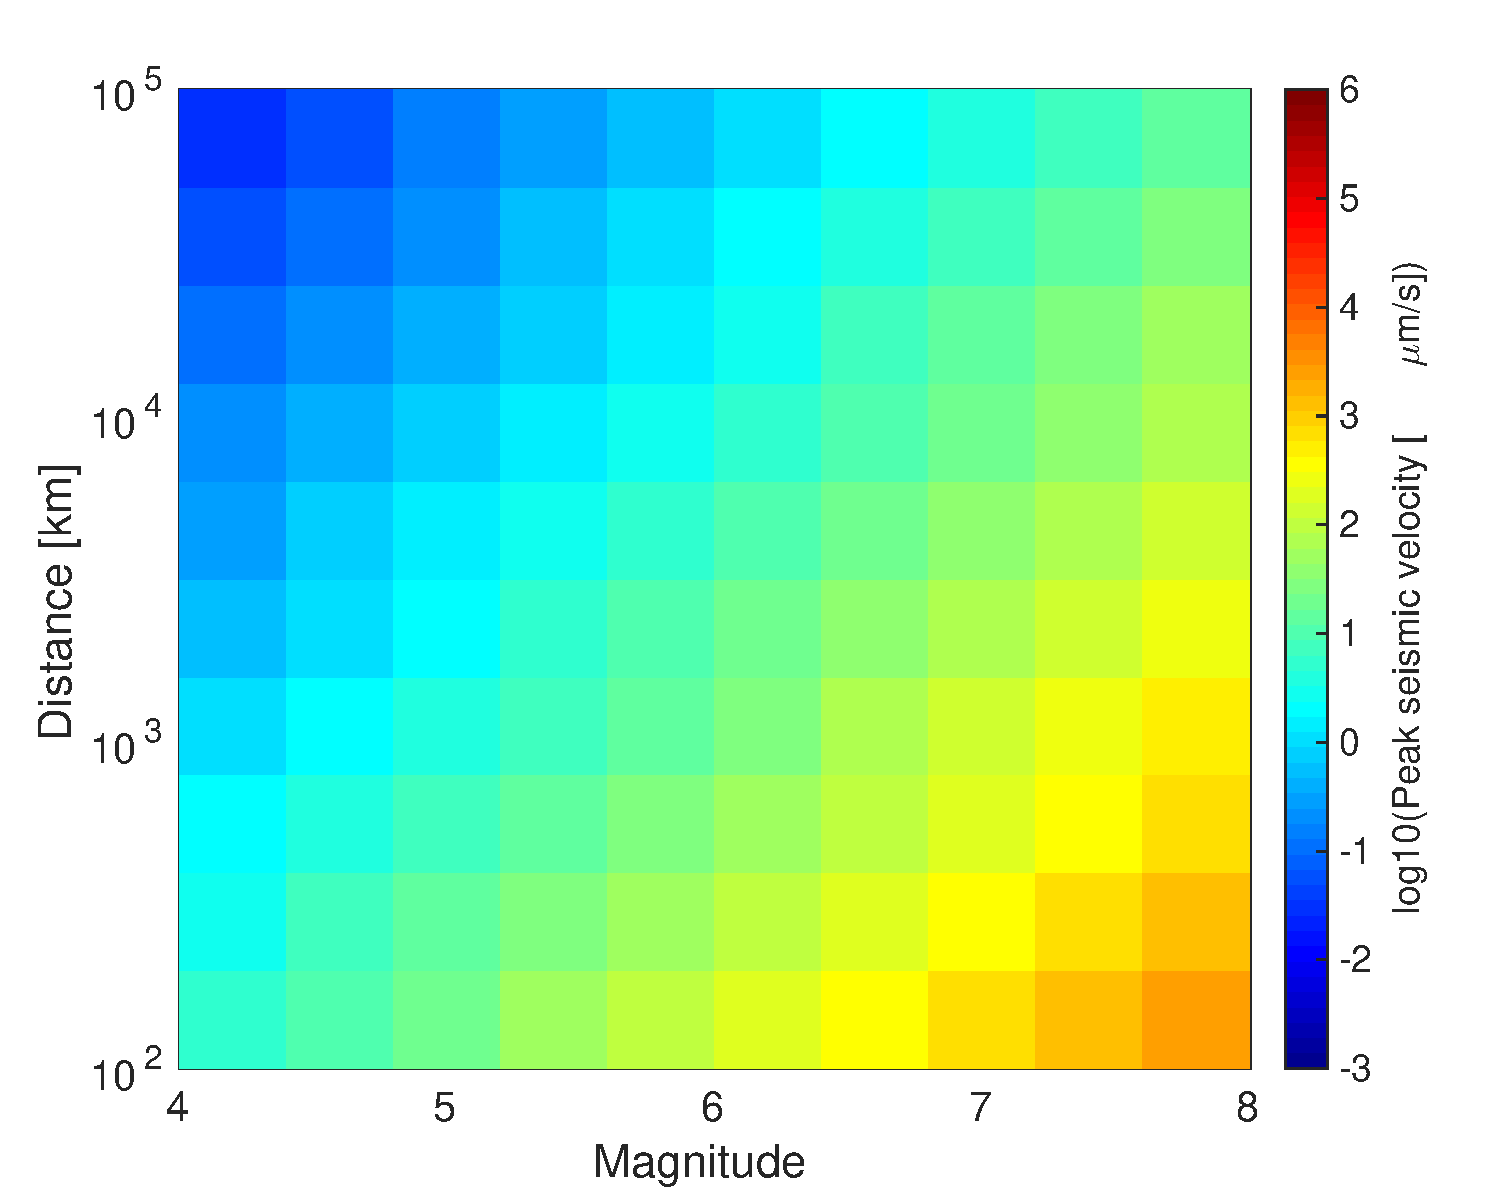
\includegraphics[width=3.5in]{LHO_M_r.pdf}
 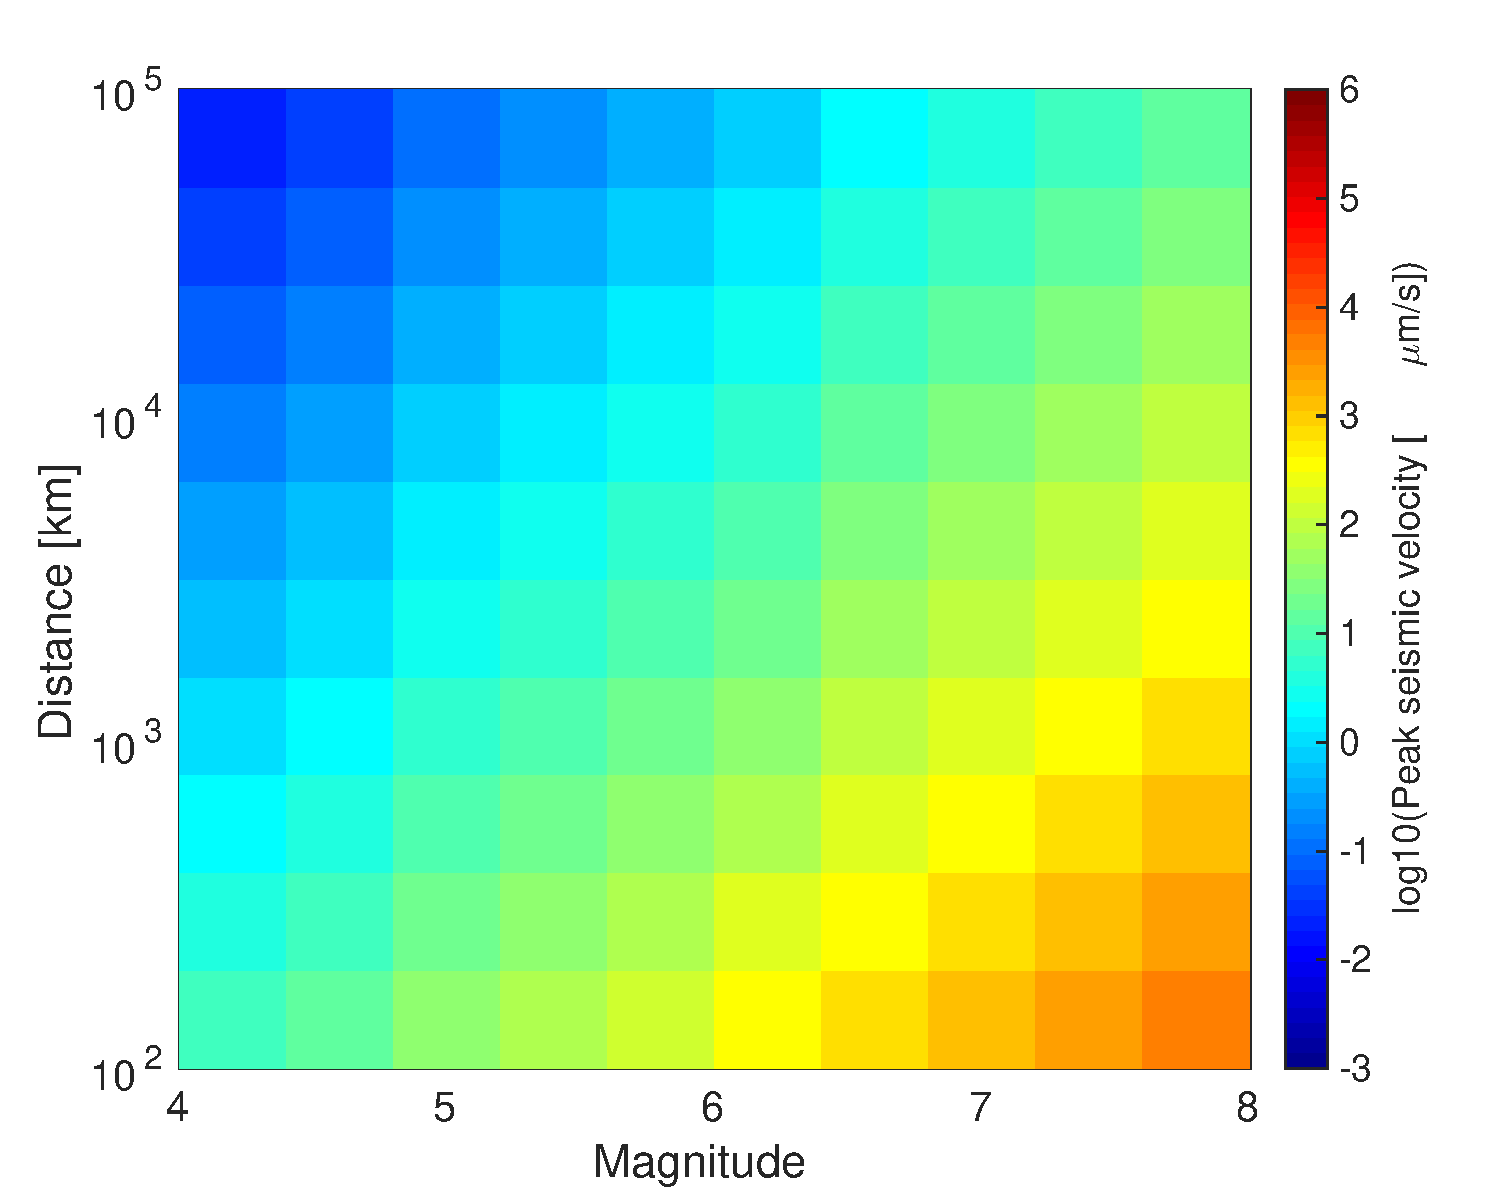
\includegraphics[width=3.5in]{LLO_M_r.pdf}
 \caption{The predicted peak ground acceleration as a function of magnitude and distance for LHO (left) and LLO (right)}
 \label{fig:MvsR}
\end{figure*}

\subsection{Epics}

The final step of the process is to use the site amplitude and time-of-arrival predictions to create warnings (and possibly detector state changes) for the detectors.
The algorithm analyzes the recent notifications and places a threshold on the predictions.
We have determined a series of three thresholds we have found useful for characterizing the potential effects on detectors.
The first is 1\,$\mu m$/s, below which we do not expect the detector sensitivity to change appreciably.
The second is 1\,$\mu m$/s to 5\,$\mu m$/s, between which we expect marginal change in detector sensitivity and potential loss of lock.
The third is 5 \,$\mu m$/s, above which we expect the detector to lose lock.

We provide an epics variable that contains the following information.
The first is the amplitude prediction for any earthquake expected to be present.
The second is where this earthquake falls on the above scale.
The third is when this earthquake is expected to arrive at the site.

\section{Performance}
\label{sec:performance}

In this section, we provide a number of metrics by which we analyze the performance of \seismon.

\subsection{Notification latency}

\begin{figure*}[t]
\hspace*{-0.5cm}
 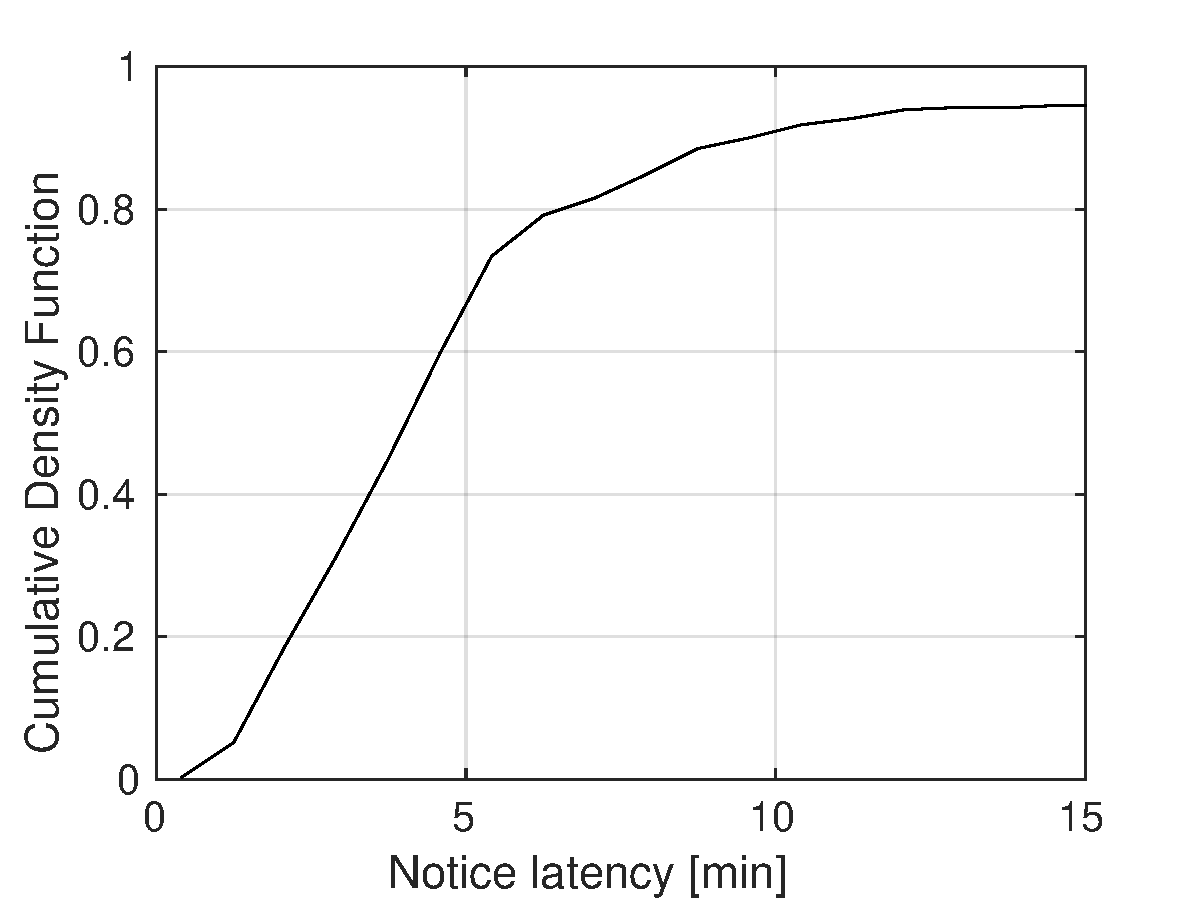
\includegraphics[width=3.5in]{earthquake_notice.pdf}
 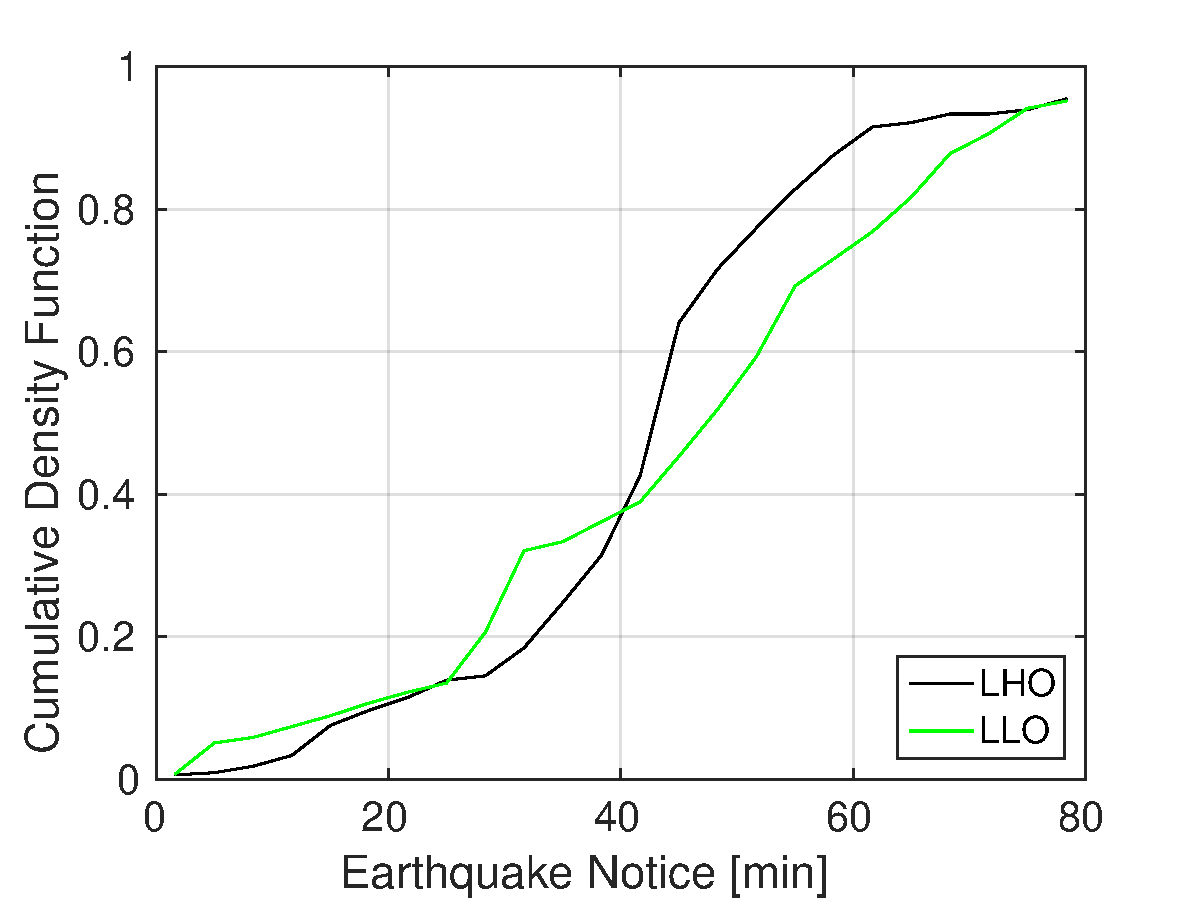
\includegraphics[width=3.5in]{lockloss_notice.pdf}
 \caption{On the left is the time delay between the earthquake and generation of the PDL client notification. On the right is the time delay between the earthquake notification from the PDL client and approximate arrival of surface waves at the LIGO Hanford site for global earthquakes. A majority of the locations allow for more than a minute of time between notification and site arrival.}
 \label{fig:delays}
\end{figure*}

One of the most important qualities of an earthquake monitor is the notification latency, or the amount of warning time a detector has to respond to incoming seismic waves.
On the left of figure~\ref{fig:delays}, we show the time delay between the earthquake and generation of the PDL client notification. In general, notices are generated within 5 minutes of the earthquake. On the right of figure~\ref{fig:delays},
the cumulative probability distribution of time delays between the earthquake and approximate arrival of surface waves, assuming surface wave velocities of 3.5\,km/s. 
In general, there is more than 10 minutes available between notification and surface wave arrivals.
This is more than sufficient time for gravitational-wave detectors to respond by changing control configurations.

\subsection{Prediction Performance}

\begin{figure}[t]
\hspace*{-0.5cm}
 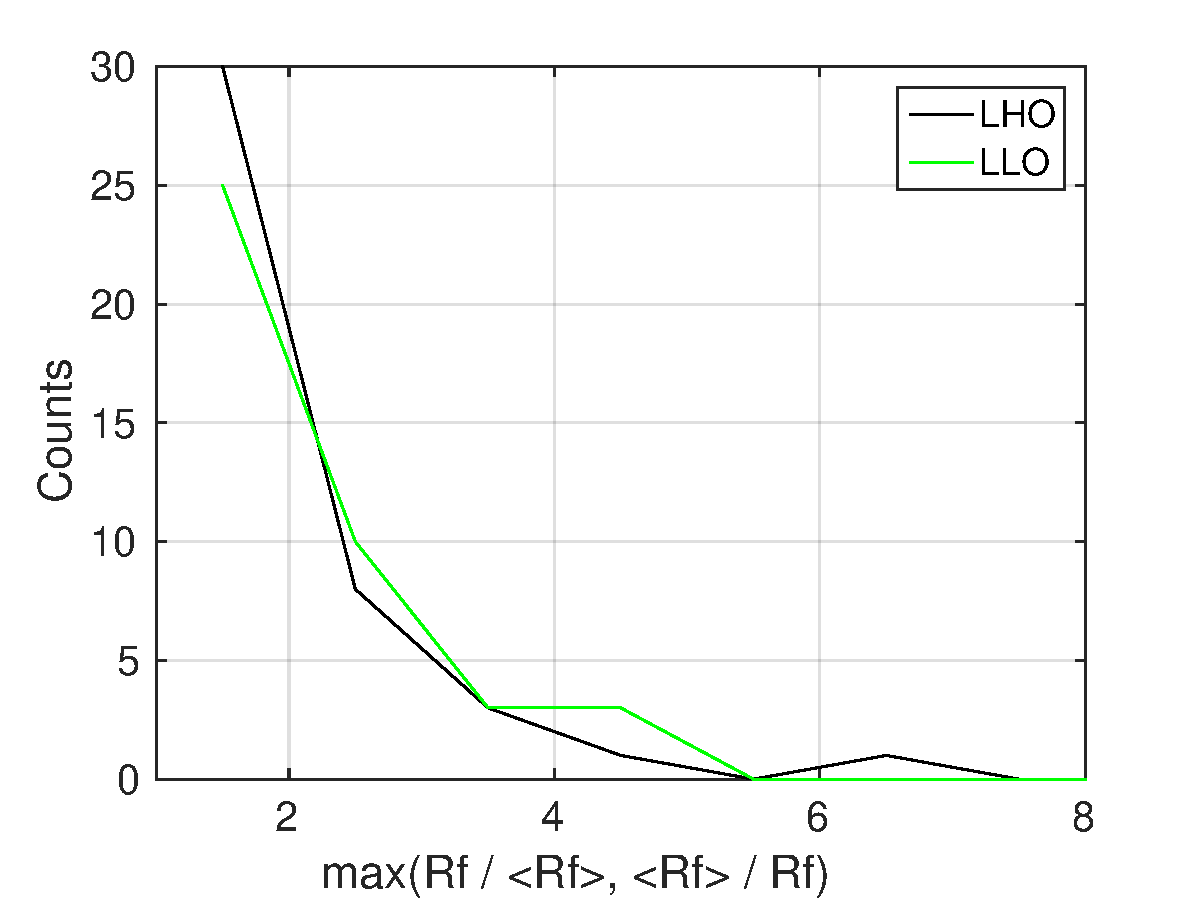
\includegraphics[width=3.5in]{pred_diff.pdf}
 \caption{Performance of estimation of peak velocities seen during O1 at the interferometers (LHO and LLO) using fit parameters estimated from S5-S6 data. About 87\% (LHO) and 94\% (LLO) of events are within a factor of 5 of the predicted value.}
 \label{fig:regressionperf}
\end{figure}

Another important quality for an earthquake monitor is the accuracy of the ground-motion amplitude prediction and the time-of-arrival.
The grond-motion amplitude performance is evaluated against the most recent science run (Observing Run 1) from September 2015 to January 2016, in Fig.\ref{fig:regressionperf}. About 94\% of events are within a factor of 5, while those that are not are almost exclusively events that are overlap of many events. This occurs often during aftershocks of large earthquakes. As the largest event is the important one, these are unimportant for predictions. There are few events that produce large surface waves without visible body waves. These are more likely to be blasts of some kind.
In some cases, there is an under-estimation of the actual seismic speeds.
This is likely due to the aliasing due to larger earthquakes, including aftershocks shortly after larger earthquakes.

\begin{figure*}[t]
\hspace*{-0.5cm}
 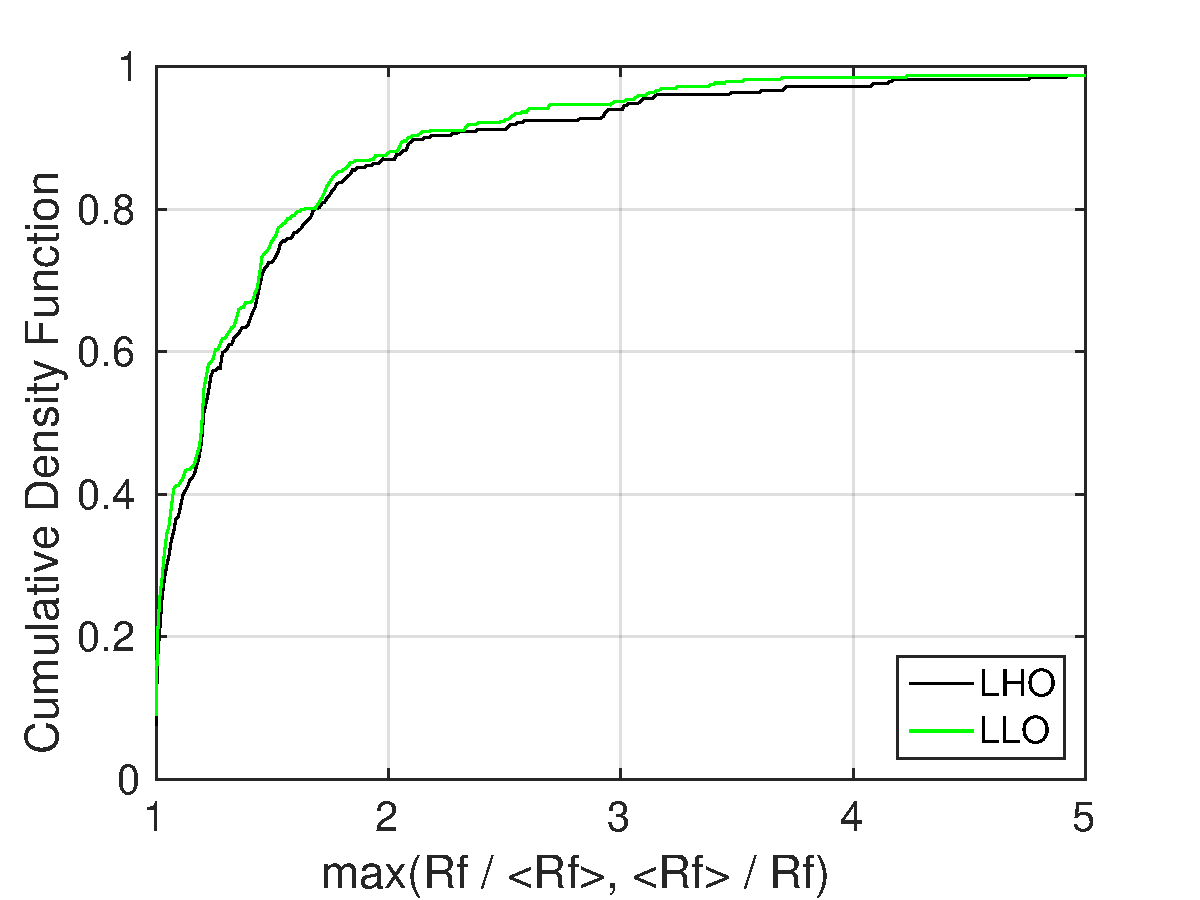
\includegraphics[width=3.5in]{initial_vs_final.pdf}
 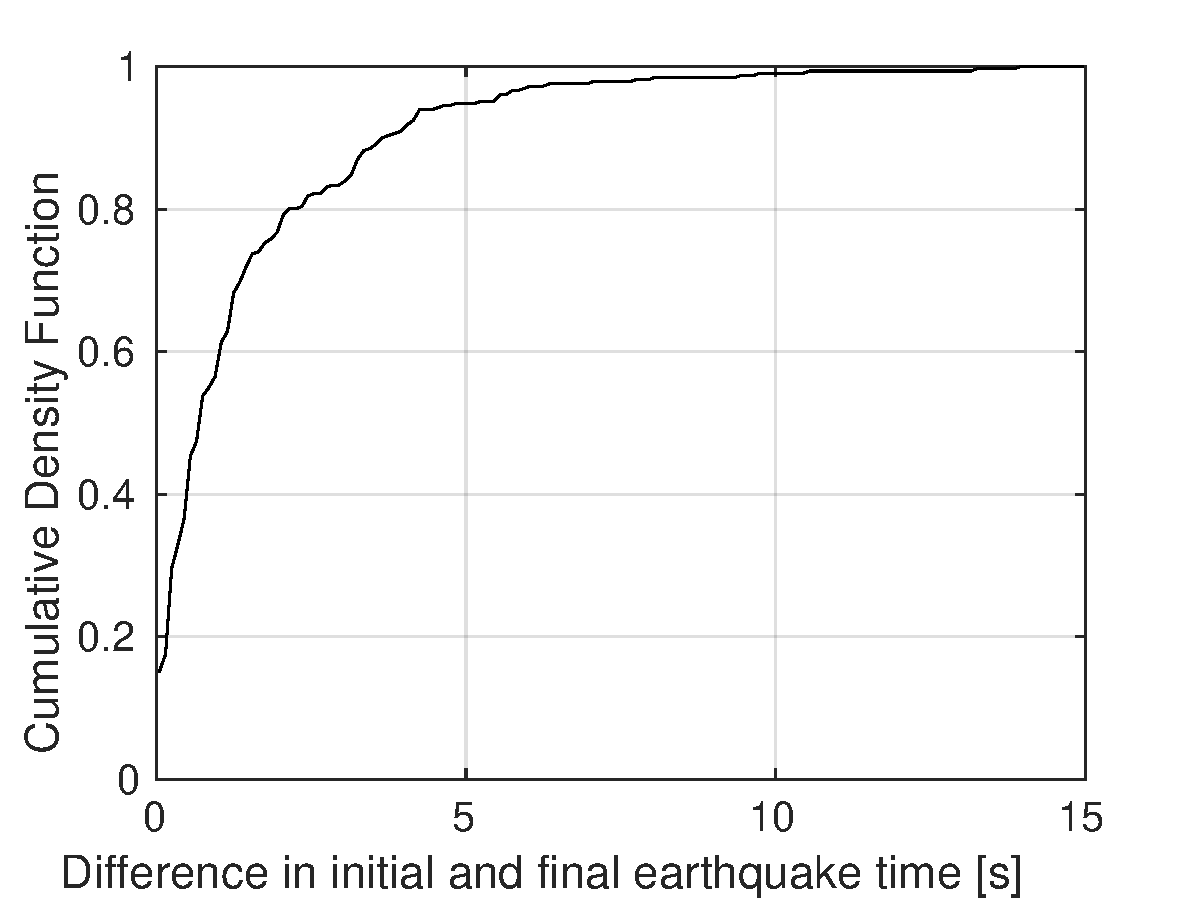
\includegraphics[width=3.5in]{lockloss_est_timediff.pdf}
 \caption{On the left is the difference of predicted peak velocities seen during O1 at the interferometers (LHO and LLO) using the initial and final estimates. About 90\% of events are within a factor of 2 of the final predicted value. On the right is the difference between the initial and final estimates of the earthquake time. About 90\% of early estimates are within 4\,s of the final time.}
 \label{fig:initialvsfinal}
\end{figure*}

As mentioned above, \seismon uses the earliest available notices for making time-of-arrival and amplitude predictions.
Because the earliest notices may only rely on a few seismometers, as well as the fact that large earthquakes do not fault all at once, the estimates for both magnitude, depth, location, and time can be off.
In Fig.\ref{fig:initialvsfinal}, we show the difference of arrival times and predicted peak velocities seen during O1 at the interferometers (LHO and LLO) using the initial and final estimates. About 90\% of events are within a factor of 2 of the final predicted value. This is a smaller error than from the regression.
In addition, we show the difference between the initial and final estimates of the earthquake time. About 90\% of early estimates are within 3\,s of the final time, which is much smaller than the latency from the generation of the notice itself.
For these reasons, the use of the early notices is not a major source of systematic error for \seismon.

\subsection{The effect of large ground velocity on gravitational-wave detectors}

\begin{figure*}[t]
\hspace*{-0.5cm}
 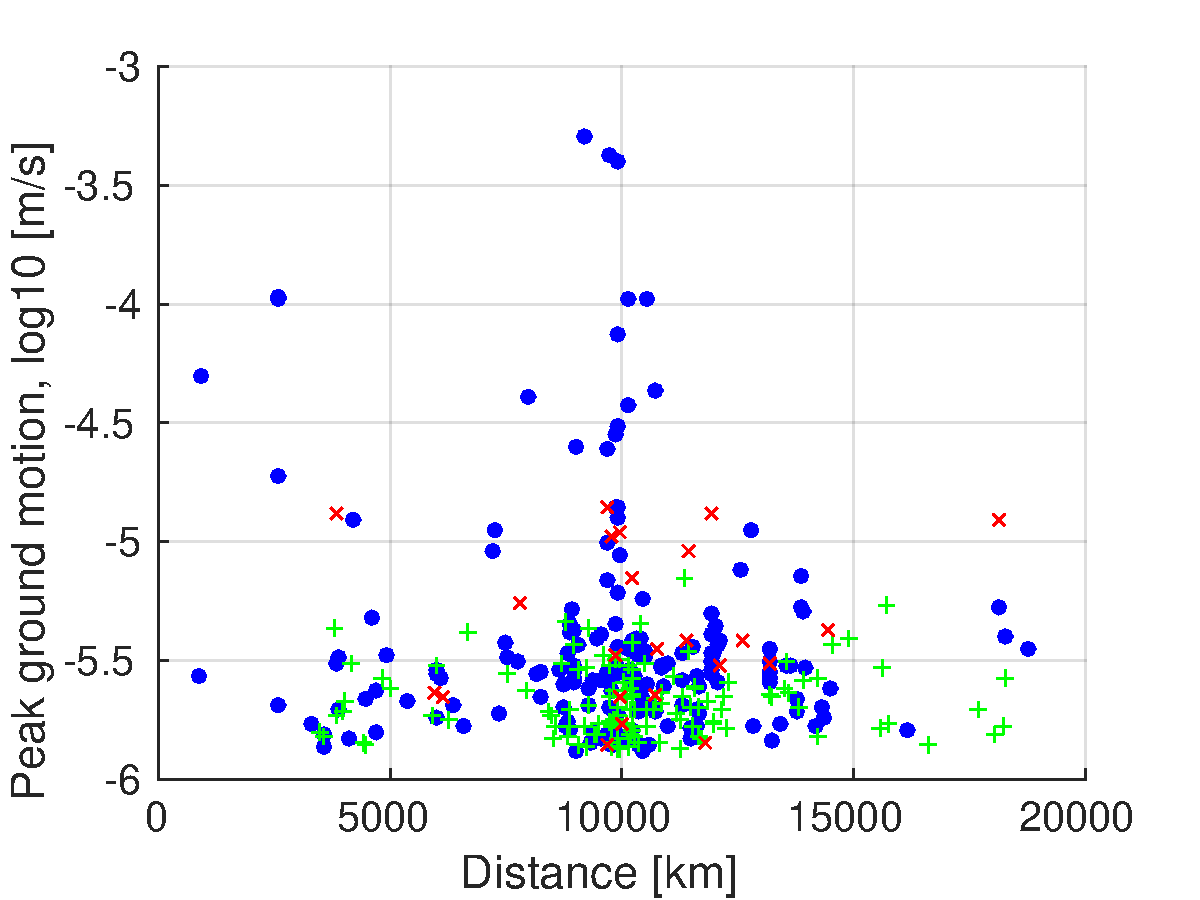
\includegraphics[width=3.5in]{lockloss_vel_distance_LHO.pdf}
  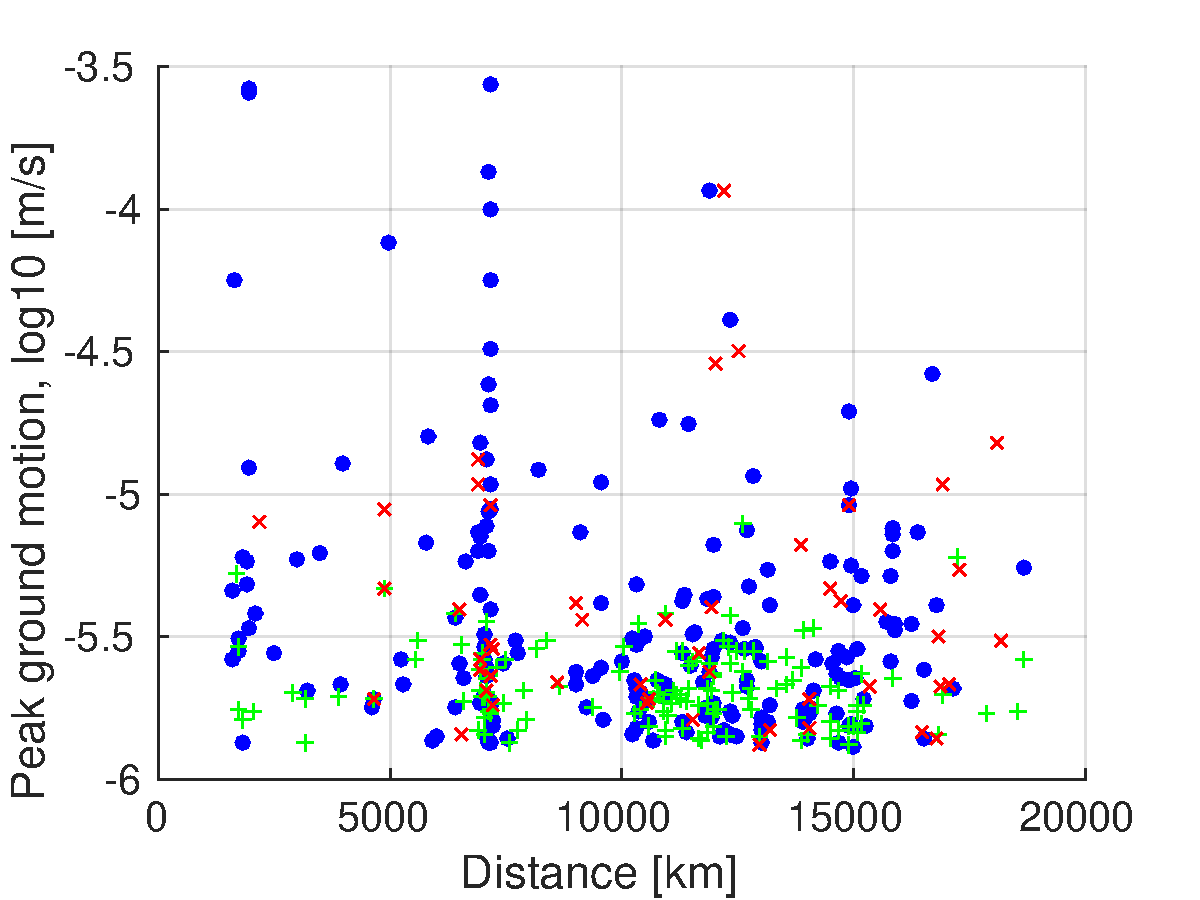
\includegraphics[width=3.5in]{lockloss_vel_distance_LLO.pdf}
 \caption{Lock loss as a function of predicted peak velocity vs. earthquake distance for the gravitational-wave detectors.}
 \label{fig:lockloss}
\end{figure*}

An earthquake monitor will only be useful for gravitational-wave detectors if it can be determined what earthquakes cause the loss of data.
We now measure the amplitude of the seismic ground motion that causes the detector to lose lock. To do so, we take all known earthquakes above magnitude 5.0 and compute their arrival times. 
We also determine the times that the gravitational-wave detectors fell out of lock during these times. 
We then compare these two figures of merit. 
Fig.~\ref{fig:lockloss} shows these times, both for those times when lock losses occurred (red), when they did not (green), and when the detector was not locked (blue). 
It is of significant interest to determine at what ground velocities the detector loses lock.
Fig.~\ref{fig:locklossCDF} shows the cumulative density function of lock loss as a function of peak ground velocity.
Lock loss typically occurs during times of ground velocities greater than about 5\,$\mu$m/s.

\begin{figure}[t]
\hspace*{-0.5cm}
  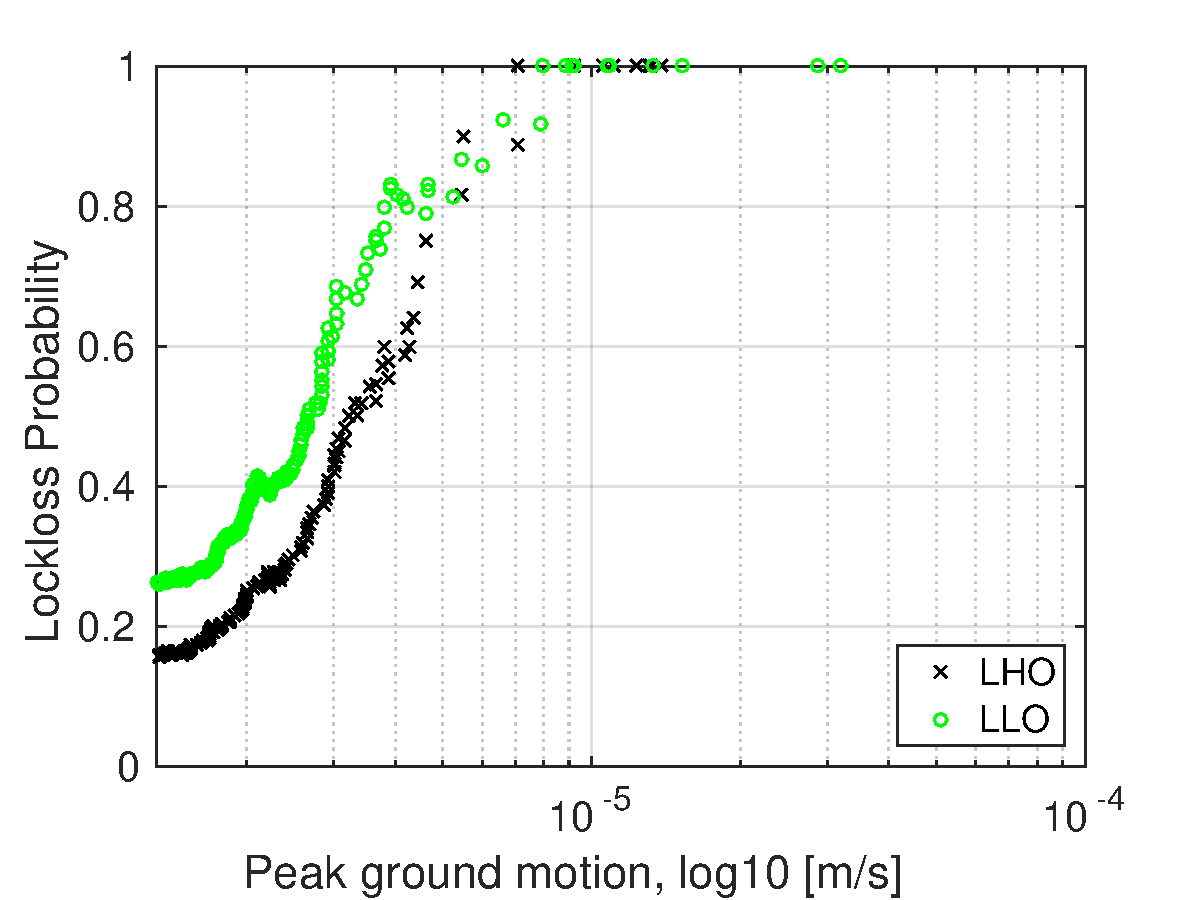
\includegraphics[width=3.5in]{lockloss_vel.pdf}
 \caption{Cumulative density function of lock loss as a function of peak ground velocity.}
 \label{fig:locklossCDF}
\end{figure}

\section{Conclusion}
\label{sec:conclusions}

In this paper, we have discussed the problem of earthquakes for gravitational-wave detectors and a pipeline designed to minimize their impact. 
We characterize this pipeline in terms of the warning time for these experiments.
We have shown that the earthquake warning system can both predict likely earthquake arrival times and ground velocity amplitudes. 

A code that performs these steps is available at https://github.com/ligovirgo/seismon/ for public download. Hopefully, this will allow other researchers to easily use the fits. Required inputs are the latitude and longitude of the site and magnitude, latitude, longitude and depth of the source.

In the future, this algorithm will be applied to the next science run. It will require coordination between the low-latency notification software and the detector control systems to maximize the utility of the system. This will include studies of the control configuration best for riding out times of large ground motion.

\section{Acknowledgments}
MC was supported by the National Science Foundation Graduate Research Fellowship
Program, under NSF grant number DGE 1144152. 
NM acknowledges Council for Science and Industrial Research (CSIR), India for providing financial support as Senior Reseach Fellow.  
LIGO was constructed by the California Institute of Technology and Massachusetts Institute of Technology with funding from the National Science Foundation and operates under cooperative agreement PHY-0757058.
This paper has been assigned LIGO document number LIGO-??????????.

%\raggedright
\bibliographystyle{unsrt}
\bibliography{references}


\end{document} 
